\documentclass[english,11pt, reqno, oneside]{amsart}
\usepackage{amsmath}
\usepackage{amssymb}
\usepackage[usenames,dvipsnames]{xcolor}
\usepackage[colorlinks=true,linkcolor=blue!95!black, citecolor = green!55!black,bookmarksdepth=3]{hyperref}
\usepackage{tikz}
\usetikzlibrary{calc}
\usetikzlibrary{math}
\usetikzlibrary{decorations.markings, decorations.pathreplacing,shapes.misc}

\begin{document}

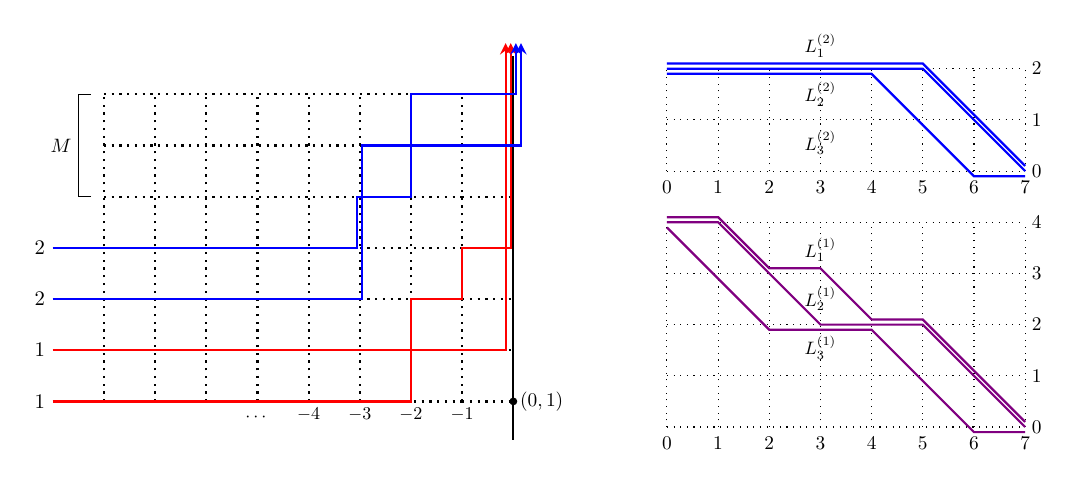
\begin{tikzpicture}[
  >=stealth,
  scale = .65]{ 

    \draw[thick] (23, -.25) -- (23, 7.25);

    \draw[black, thick, dotted] (15, .5) -- (15, 6.5);
    \draw[black, thick, dotted] (16, .5) -- (16, 6.5);
    \draw[black, thick, dotted] (17, .5)  -- (17, 6.5);
    \draw[black, thick, dotted] (18, .5) node[below = 2, scale = .65]{$\cdots$} -- (18, 6.5);
    \draw[black, thick, dotted] (19, .5) node[below, scale = .65]{$-4$}  -- (19, 6.5);
    \draw[black, thick, dotted] (20, .5) node[below, scale = .65]{$-3$} -- (20, 6.5);
    \draw[black, thick, dotted] (21, .5) node[below, scale = .65]{$-2$} -- (21, 6.5);
    \draw[black, thick, dotted] (22, .5) node[below, scale = .65]{$-1$} -- (22, 6.5);

    \draw[black, thick, dotted] (15, .5) -- (22, .5);
    \draw[black, thick, dotted] (15, 1.5) -- (22, 1.5);
    \draw[black, thick, dotted] (15, 2.5) -- (22, 2.5);
    \draw[black, thick, dotted] (15, 3.5) -- (22, 3.5);
    \draw[black, thick, dotted] (15, 4.5) -- (22, 4.5);
    \draw[black, thick, dotted] (15, 5.5) -- (22, 5.5);
    \draw[black, thick, dotted] (15, 6.5) -- (22, 6.5);

    \draw[thick, dotted] (22, 2.5) -- (23, 2.5);
    \draw[thick, dotted] (22, 4.5) -- (23, 4.5);
    \draw[thick, dotted] (22, .5) -- (23, .5);
    \draw[thick, dotted] (22, 1.5) -- (23, 1.5);

    \draw[->, red, thick] (14, .5) node[left, scale = .75, black]{$1$} -- ++(1, 0) -- ++(6, 0) -- ++(0, 1) -- ++(1.85, 0) -- ++(0, 6);
    \draw[->, red, thick] (14, 1.5) node[left, scale = .75, black]{$1$} -- ++(1, 0) -- ++(6, 0) -- ++(0, 1) -- ++(1, 0) -- ++(0, 1) -- ++(0.95, 0) -- ++(0, 4);
    \draw[->, blue, thick] (14, 2.5) node[left, scale = .75, black]{$2$} -- ++(1, 0) -- ++(5.05, 0) -- ++(0, 3) -- ++(0.95, 0) -- ++(0, 1) -- ++(1, 0) -- ++(1.05, 0) -- ++(0, 1);
    \draw[->, blue, thick] (14, 3.5) node[left, scale = .75, black]{$2$} -- (15, 3.5) -- (19.95, 3.5) -- (19.95, 4.5) -- (21, 4.5) -- (21, 5.5) -- (23.15, 5.5) -- (23.15, 7.5);

    \draw[-] (14.75, 4.5) -- (14.5, 4.5) -- (14.5, 6.5) -- (14.75, 6.5);
    \draw[] (14.5, 5.5) circle [radius = 0] node[left, scale = .7]{$M$};


    \node[circle, fill, inner sep = 1pt] at (23, 0.5) {};
    \node[anchor=west, scale=0.7] at (23,0.5) {$(0,1)$};


    \foreach \x in {0,...,4}
      \draw[dotted] (26, \x) -- ++(7, 0) node[right, scale = .7]{$\x$};

    \foreach \x in {0,...,7}
      \draw[dotted] (26+\x, 0) node[below = 1, scale = .7]{$\x$} -- ++(0, 4);

    \foreach \x in {0,...,2}
      \draw[dotted] (26, 5+\x) -- ++(7, 0) node[right, scale = .7]{$\x$};

    \foreach \x in {0,...,7}
      \draw[dotted] (26+\x, 5) node[below = 1, scale = .7]{$\x$} -- ++(0, 2);


    \draw[ thick, blue] (26, 7.1) -- (31, 7.1) -- (33, 5.1);
    \draw[ thick, blue] (26, 7) -- (31, 7) -- (33, 5);
    \draw[ thick, blue] (26, 6.9) -- (30, 6.9) -- (32, 4.9) -- (33, 4.9);


    \draw[ thick, violet] (26, 4.1) -- ++(1, 0) -- ++(1, -1) -- ++(1, 0) -- ++(1, -1) -- ++(1, 0) -- ++(1, -1) -- ++(1, -1);
    \draw[ thick, violet] (26, 4) -- (27, 4) -- (28, 3) -- (29, 2) -- (31, 2) -- (32, 1) -- (33, 0);
    \draw[ thick, violet] (26, 3.9) -- (27, 2.9) -- (28, 1.9) -- (29, 1.9) -- (30, 1.9) -- (31, .9) -- (32, -.1) -- (33, -.1);

    \draw[] (29, 7.1) circle [radius = 0] node[above, scale = .65]{$L_1^{(2)}$};
    \draw[] (29, 6.5) circle [radius = 0] node[scale = .65]{$L_2^{(2)}$};
    \draw[] (29, 5.9) circle [radius = 0] node[below, scale = .65]{$L_3^{(2)}$};

    \draw[] (29, 3.1) circle [radius = 0] node[above, scale = .65]{$L_1^{(1)}$};
    \draw[] (29, 2.5) circle [radius = 0] node[scale = .65]{$L_2^{(1)}$};
    \draw[] (29, 1.9) circle [radius = 0] node[below, scale = .65]{$L_3^{(1)}$};
  }
\end{tikzpicture}

\end{document}